% EACL 2027 Industry Track submission - Vyuha
% Overleaf setup: use the official ACL template (https://github.com/acl-org/acl-style-files).
% Place acl.sty and acl_natbib.bst in the project. Do NOT modify the style files.
% This draft is ANONYMISED for double-blind review (no author names; repo links anonymised).
% Content target: <= 6 pages (References, Limitations, Ethics, Appendix do NOT count).
\documentclass[11pt]{article}
\usepackage[review]{acl}          % 'review' -> line numbers + anonymised
\usepackage{times}
\usepackage{latexsym}
\usepackage{booktabs}
\usepackage{graphicx}
\usepackage{amsmath}
\usepackage[T1]{fontenc}
\usepackage[utf8]{inputenc}
\usepackage{microtype}
\usepackage{tikz}
\usetikzlibrary{positioning,arrows.meta}
\usepackage{pgfplots}
\pgfplotsset{compat=1.18}
\usepackage{url}

\title{Vyuha: A Reproducible, Free-Compute Layered Guardrail for Deploying\\
LLM Defenses --- and How to Measure One Honestly}

% --- anonymised for review ---
\author{Anonymous EACL submission}

\begin{document}
\maketitle

\begin{abstract}
Prompt injection is the top risk in the OWASP Top~10 for LLM Applications, and recent
adaptive-attack work shows any single filter, once known, can be evaded --- ``the attacker moves
second.'' Yet most guard evaluations run on balanced laboratory sets, not deployment conditions.
We present \textbf{Vyuha}, a defense-in-depth guardrail that composes six independent layers
(normalisation, a CPU fast detector, a content guard, agent/tool-injection defense, output
moderation, and continuous red-teaming) and ships as a library, a service, and a CLI. Our
contribution is not a new algorithm but a \emph{deployable composition}, an
\emph{evaluation methodology} suited to LLM-guard components (recall-first, confidence intervals,
adaptive-attack ablation, a standardised-benchmark reconstruction, and base-rate discipline), and
\emph{full reproducibility on a single free GPU}. We report security-grade metrics with 95\%
confidence intervals: the CPU fast layer matches a GPU neural guard's obfuscation robustness at
$\sim$8\,ms; against an adaptive attacker, normalisation alone leaves ASR at 1.00 while adversarial
augmentation closes it to 0.03 at 1\% false-positive rate; on a NIST-AI-RMF guard benchmark our
0.6B content guard reaches 0.886 recall on complete-harmful-request axes --- on par with a 7$\times$
larger model; and a session-level monitor catches 71\% of multi-turn (Crescendo) escalations a
per-message moderator catches 0\% of. We are explicit throughout about where stronger
(white-box, formally verified, or paid-compute) work exists.
\end{abstract}

\section{Introduction}
Large language models deployed as assistants and autonomous agents face a moving adversary:
jailbreaks that strip safety behaviour, prompt injections hidden in retrieved content and tool
metadata, obfuscated and multilingual attacks, semantic (persuasion) attacks with no surface tell,
and responses that leak secrets. Prompt injection is the \#1 risk in the OWASP Top~10 for LLM
Applications \citep{owasp-llm}, and \citet{attacker-second} show that adaptive attackers bypass a
dozen recent defenses at $>$90\% attack-success-rate (ASR) by tuning general optimisers: robustness
must be \emph{measured}, not assumed.

Two deployment realities are under-served by current practice. First, guards are typically evaluated
on balanced attack/benign sets, whereas production traffic is overwhelmingly benign, so the
false-positive rate dominates cost. Second, single-message moderation is the norm, yet multi-turn
(Crescendo) attacks \citep{crescendo} escalate across turns while every individual turn stays benign.

We present \textbf{Vyuha}, a layered guardrail built under one operating constraint --- it must train
and run on a single free GPU --- so that every number is reproducible without a lab budget. Our
contributions are: (1) a \emph{deployable} six-layer composition (library, service, CLI) with a
selective cascade that keeps the expensive guard off the hot path; (2) an \emph{evaluation
methodology} for LLM-guard components --- recall-first, with Wilson confidence intervals, an
adaptive-attack ablation, a standardised-benchmark reconstruction, and base-rate and contamination
discipline; and (3) an honest account, at every layer, of where stronger work exists. No single
component is a new algorithm; the contribution is the measured composition and its reproducibility.

\begin{figure*}[t]
\centering
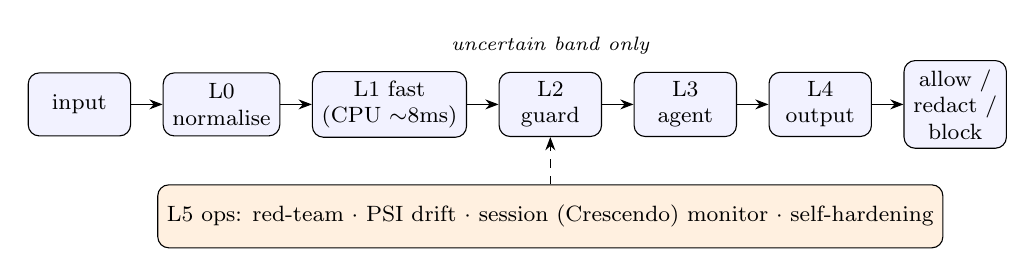
\begin{tikzpicture}[font=\footnotesize, >=Stealth,
  box/.style={draw, rounded corners, minimum height=8mm, minimum width=13mm, align=center, fill=blue!5}]
\node[box] (in) {input};
\node[box, right=4mm of in] (l0) {L0\\normalise};
\node[box, right=4mm of l0] (l1) {L1 fast\\(CPU $\sim$8ms)};
\node[box, right=4mm of l1] (l2) {L2\\guard};
\node[box, right=4mm of l2] (l3) {L3\\agent};
\node[box, right=4mm of l3] (l4) {L4\\output};
\node[box, right=4mm of l4] (out) {allow /\\redact /\\block};
\foreach \a/\b in {in/l0, l0/l1, l1/l2, l2/l3, l3/l4, l4/out} \draw[->] (\a)--(\b);
\node[above=1mm of l2, font=\scriptsize\itshape] {uncertain band only};
\node[box, fill=orange!12, below=6mm of l2, minimum width=40mm] (l5)
  {L5 ops: red-team $\cdot$ PSI drift $\cdot$ session (Crescendo) monitor $\cdot$ self-hardening};
\draw[->, dashed] (l5.north) -- (l2.south);
\end{tikzpicture}
\caption{The Vyuha cascade. The CPU fast layer (L1) triages the majority of traffic; the expensive
content guard (L2) is consulted only on the uncertain band; L3 defends the agent/tool path; L4 gates
egress; and L5 continuously red-teams and monitors.}
\label{fig:arch}
\end{figure*}

\section{The Vyuha System}
Vyuha is a pipeline of six layers (Figure~\ref{fig:arch}), each owning a different failure mode and
escalating only when needed (a \emph{selective cascade} that keeps per-request cost low).

\paragraph{L0 --- Normalisation.} De-obfuscation (Unicode NFKC, Base64/ROT13 decode-and-rescreen,
homoglyph mapping, zero-width/bidi stripping) plus an \emph{adaptive multi-view de-spacing} routine
that detects letter-gap width dynamically. This is rule-based, deterministic, and free.

\paragraph{L1 --- Fast detector (RJD-v2).} An always-on CPU triage ($\sim$8\,ms/prompt):
TF-IDF char+word n-grams, engineered features, and a calibrated ensemble, trained with adversarial
augmentation. It decides the majority of traffic so the expensive guard is consulted only on the
uncertain band.

\paragraph{L2 --- Content guard.} For harmful-topic and semantic coverage we \emph{compose} an open
content guard (Qwen3Guard-0.6B), invoked on the cascade's uncertain band. We do not out-build mature
content guards; the stack's semantic coverage is the composed guard's.

\paragraph{L3 --- Agent defense.} An injection scanner de-obfuscates and sanitises untrusted tool
outputs; an \emph{MCP tool-poisoning scanner} screens tool \emph{descriptions/metadata} at
registration time; a tool policy enforces an instruction hierarchy (system\,$>$\,user\,$>$\,tool),
hard-blocking a dangerous action that appears on a tainted turn and was not in the user's stated
intent. This is a free-compute, black-box approximation of capability-based defenses such as CaMeL
\citep{camel}, and we say so.

\paragraph{L4 --- Output moderation.} An egress gate that redacts PII, blocks secret/credential and
system-prompt/canary leakage, and scores response harm with the content guard on the
(prompt, response) pair.

\paragraph{L5 --- Continuous ops.} An automated red-team (public attacks only), a population drift
monitor, a session-level escalation monitor for Crescendo, and a self-hardening loop.

\section{Evaluation Methodology}
Deploying LLM-based guards changes what a credible evaluation looks like; we adopt five practices.
\textbf{(1) Recall-first.} A missed harmful item costs more than a false positive, so recall is the
headline metric \citep{guard-bench}, reported at a fixed low false-positive rate rather than at a
default threshold. \textbf{(2) Confidence intervals.} Every headline proportion is reported with a
Wilson 95\% interval, which keeps small-$n$ claims honest (a ``perfect'' 1.00 on $n{=}5$ has a wide
interval). \textbf{(3) Adaptive-attack ablation.} We measure against an attacker that searches over
compositions of known evasions --- both an exhaustive pairwise sweep and a harder genetic
(deep-chain, crossover) search over the same public transforms --- and ablate each design choice,
rather than reporting a static per-mutator number that understates the attack surface. \textbf{(4) Standardised benchmark.} We score
the content guard on the 8 NIST-AI-RMF safety categories following \citet{guard-bench}.
\textbf{(5) Base-rate and contamination discipline.} Benign controls are drawn from real user
prompts; benchmark sets are held test-only. All numbers reproduce from public notebooks on a single
Kaggle T4.

\section{Results}
Table~\ref{tab:main} summarises the measured results; all proportions carry 95\% confidence intervals.

\begin{table}[t]
\centering\small
\begin{tabular}{@{}lll@{}}
\toprule
\textbf{Axis (layer)} & \textbf{Metric} & \textbf{Result} \\
\midrule
Obfuscation (L1) & recall & \textbf{1.00} incl.\ held-out \\
 & latency & $\sim$8\,ms CPU \\
Adaptive (L1) & ASR, L0 only & 1.00 [0.97,1.00] \\
 & ASR, L0+aug (pairwise) & \textbf{0.03} [0.01,0.08] \\
 & ASR, L0+aug (genetic) & \textbf{0.07} [0.04,0.12] \\
Semantic (L2) & PAIR recall & \textbf{0.90} (L1: 0.07) \\
NIST-RMF (L2) & recall, req.\ axes & \textbf{0.886} ($\approx$4B: 0.84) \\
 & benign FPR & 0.071 \\
Agent inj.\ (L3) & AgentDojo ASR & 1.00\,$\rightarrow$\,\textbf{0.00} \\
MCP poison (L3) & detection & \textbf{1.00} [0.87,1.00] \\
Multi-turn (L5) & session detect & \textbf{0.71} [0.65,0.77] \\
 & per-message & 0.00 \\
Output (L4) & leak/harm F1 & \textbf{1.00} \\
\bottomrule
\end{tabular}
\caption{Vyuha, security-grade metrics with 95\% CIs. Every value reproduces from public notebooks
on a single free GPU.}
\label{tab:main}
\end{table}

\paragraph{Obfuscation is closed cheaply (C1).} RJD-v2 reaches ROC-AUC 0.923, recall@1\%FPR 0.330,
over-refusal 0.044 at $\sim$8\,ms on CPU --- matching a GPU DeBERTa injection guard (0.896 / 0.113)
at $\sim$8$\times$ lower latency and lower over-refusal. Recall under attack is 1.00 on Base64, ROT13,
character-spacing and a \emph{held-out} wider-spacing variant; the adaptive de-spacing fix closed the
character-spacing gap from ASR 0.83 to 0.00 and generalises to the held-out variant.

\begin{figure}[t]
\centering
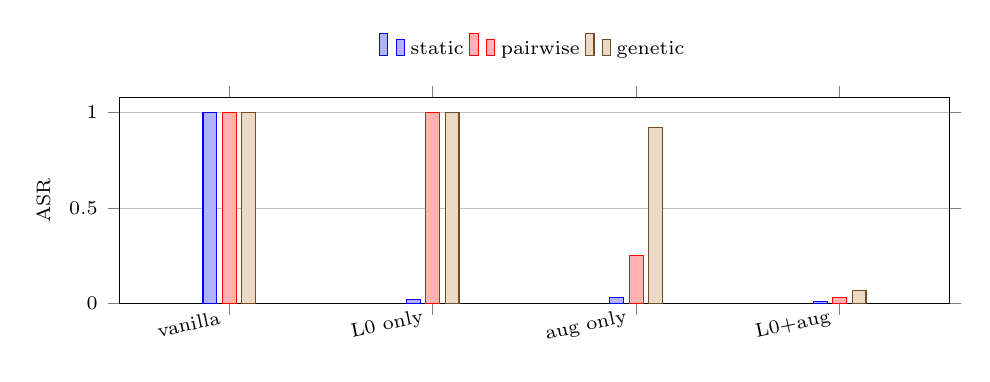
\begin{tikzpicture}
\begin{axis}[ybar, width=\columnwidth, height=4.2cm, font=\scriptsize, bar width=5pt,
  ymin=0, ymax=1.08, ylabel={ASR}, symbolic x coords={vanilla,L0 only,aug only,L0+aug},
  xtick=data, x tick label style={rotate=12,anchor=east}, ymajorgrids, tick align=outside,
  enlarge x limits=0.18, legend style={at={(0.5,1.13)},anchor=south,legend columns=3,draw=none}]
\addplot coordinates {(vanilla,1.00)(L0 only,0.02)(aug only,0.03)(L0+aug,0.01)};
\addplot coordinates {(vanilla,1.00)(L0 only,1.00)(aug only,0.25)(L0+aug,0.03)};
\addplot coordinates {(vanilla,1.00)(L0 only,1.00)(aug only,0.92)(L0+aug,0.07)};
\legend{static,pairwise,genetic}
\end{axis}
\end{tikzpicture}
\caption{Adaptive-attack ablation (C4), 150 in-the-wild seeds. L0 alone cuts \emph{static} ASR to 0.02
but both adaptive attackers still reach 1.00. Only the full detector (L0+aug) holds --- 0.03 [0.01,0.08]
pairwise and 0.07 [0.04,0.12] under a harder genetic search --- while augmentation \emph{alone}
collapses to 0.92 under the genetic attacker, showing L0 and augmentation are both load-bearing.}
\label{fig:adaptive}
\end{figure}

\paragraph{Adaptive robustness (C4).} Figure~\ref{fig:adaptive} shows the ablation. Against an adaptive attacker (exhaustive search over 101
single/paired evasions per seed) on 150 real in-the-wild jailbreak seeds: a bare detector is fully
evaded (1.00). Normalisation alone drops the \emph{static} per-mutator ASR to 0.02 yet the adaptive
attacker still reaches 1.00 [0.97,1.00] --- a $+0.98$ ``attacker-moves-second'' premium the static
number hides. Adversarial augmentation is the load-bearing fix: the full detector holds adaptive ASR
to 0.03 [0.01,0.08] at 1\% benign FPR. A harder \emph{genetic} attacker (deep transform chains with
crossover, $\sim$110 queries/seed) confirms this rather than breaking it --- the full detector holds at
0.07 [0.04,0.12], statistically indistinguishable from the pairwise 0.03. The same genetic search,
however, drives \emph{augmentation-alone} from 0.25 to 0.92 [0.86,0.95]: L0 normalisation is far more
load-bearing than the pairwise ablation implied, and neither component is sufficient on its own --- both
earn their place.

\paragraph{Division of labour (L1 vs L2).} On 103 real PAIR jailbreaks the surface detector flags
6.8\% (no surface tell) while the composed content guard flags 90.3\% at 4.8\% over-refusal ---
semantics are, by design, L2's job, not L1's.

\begin{figure}[t]
\centering
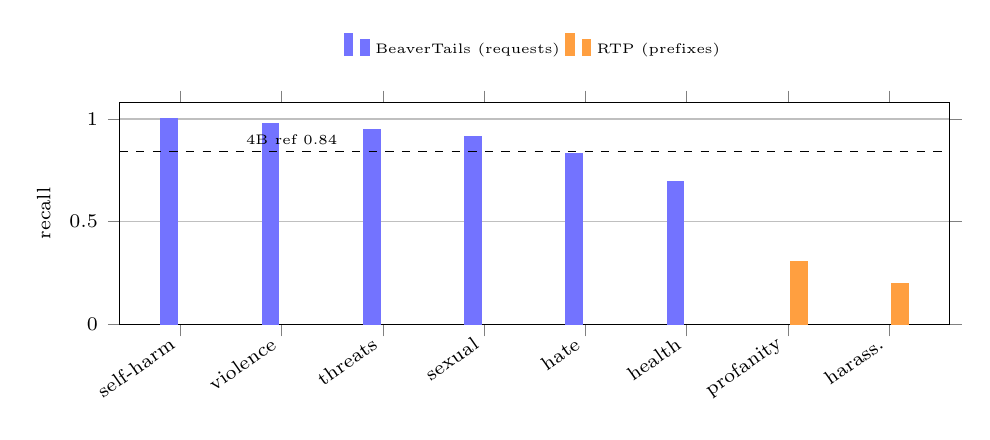
\begin{tikzpicture}
\begin{axis}[ybar, width=\columnwidth, height=4.4cm, font=\scriptsize, bar width=6pt,
  ymin=0, ymax=1.08, ylabel={recall}, xmin=0.4, xmax=8.6, xtick={1,2,3,4,5,6,7,8},
  xticklabels={self-harm,violence,threats,sexual,hate,health,profanity,harass.},
  x tick label style={rotate=35,anchor=east}, ymajorgrids, tick align=outside,
  legend style={at={(0.5,1.15)},anchor=south,legend columns=2,draw=none,font=\tiny}]
\addplot[fill=blue!55,draw=blue!55] coordinates {(1,1.00)(2,0.980)(3,0.950)(4,0.916)(5,0.833)(6,0.696)};
\addplot[fill=orange!75,draw=orange!75] coordinates {(7,0.307)(8,0.200)};
\draw[dashed] (axis cs:0.4,0.84) -- (axis cs:8.6,0.84);
\node[font=\tiny] at (axis cs:2.1,0.90) {4B ref 0.84};
\legend{BeaverTails (requests),RTP (prefixes)}
\end{axis}
\end{tikzpicture}
\caption{NIST-RMF per-category recall (Qwen3Guard-0.6B). On complete-harmful-request axes
(BeaverTails) it meets or exceeds the benchmark's 4B leader (0.84, dashed); the two toxicity-prefix
axes (RealToxicityPrompts) are short fragments a request-focused guard flags less.}
\label{fig:nist}
\end{figure}

\paragraph{NIST-AI-RMF guard benchmark (L2).} Figure~\ref{fig:nist} shows the per-category split. Scoring the 0.6B content guard on the 8 NIST-AI-RMF
categories \citep{guard-bench} (a reconstruction from BeaverTails and RealToxicityPrompts;
807 unsafe / 800 benign; not the official split): scoring the guard's continuous $P(\text{unsafe})$,
recall is 0.886 on the six complete-harmful-request axes at 7.1\% benign FPR --- on par with the
benchmark's best model (Qwen Guard 4B, 0.840) despite being $\sim$7$\times$ smaller --- and 0.253 on
the two toxicity-prefix axes (short fragments a request-focused guard flags less), for an aggregate
0.651 [0.62,0.68]. A small guard is competitive with a much larger one on complete harmful requests;
the per-category spread is why L2 composes guards. The complementary guard (Granite Guardian) has
higher recall (0.931 on the six axes) but over-flags this benign set badly (63.8\% FPR), so it is not
deployable alone --- and a raw OR at threshold 0.5 inherits that (recall 0.832 at 0.64 FPR). Calibrated
instead on each guard's continuous score to a fixed per-member FPR, the union \emph{does} confirm the
benchmark's ensembling recommendation where it matters: at a strict $\sim$2\% union FPR it lifts recall
to 0.261 versus 0.097 for the single guard (a $2.7\times$ gain), and 0.413 vs.\ 0.169 at $\sim$4\%,
the advantage narrowing as FPR rises and vanishing by $\sim$16\%. The lesson is operational: a
deployable union must run on calibrated continuous scores at per-member thresholds, never a raw OR, and
its value is concentrated at the low-FPR operating point production actually uses.

\paragraph{Agent and multi-turn defense (L3, L5).} On AgentDojo (banking, \emph{important\_instructions}),
L3 drives injection ASR to 0.00 on both a weak and a strong open agent; injection-under-obfuscation
detection is 1.00 versus 0.00--0.17 for a regex baseline. The MCP scanner detects 1.00 [0.87,1.00] of
poisoned tool metadata at zero false positives on 25 poisoned / 27 benign tools. The session-level
monitor flags 71\% [0.65,0.77] of modeled Crescendo escalations at 0\% benign FPR, versus 0\% for a
per-message moderator (every turn stays sub-threshold).

\section{Deployment and Governance}
Vyuha ships as a Python library, a FastAPI service (\texttt{/scan}, \texttt{/moderate},
\texttt{/guard\_turn}), and a CLI, so a team can place it in front of or behind an LLM with a few
lines of code.

\paragraph{Cost.} The selective cascade bounds per-request cost. The CPU fast layer ($\sim$8\,ms)
decides the majority of traffic, and the GPU content guard runs only on the uncertain band, so the
expected guard cost per request scales with the \emph{uncertain-band rate} rather than with total
traffic --- the lever a deployment actually controls. Because production traffic is overwhelmingly
benign, thresholds are set at a fixed low false-positive rate, where a small change in FPR dominates
total operating cost; recall is then reported at that operating point rather than at a default 0.5.

\paragraph{Governance.} Layers map onto the OWASP LLM Top~10 and the NIST AI RMF Measure/Manage
functions (Table~\ref{tab:gov}); risks outside scope are named rather than papered over. Continuous
red-teaming, the PSI drift monitor, and the self-hardening loop support lifecycle maintenance as the
attack mix shifts --- the operational-maturity concern this track foregrounds --- and every reported
number is regenerable from versioned public notebooks, giving a simple audit trail.

\begin{table}[t]\centering\small
\begin{tabular}{@{}ll@{}}
\toprule
\textbf{OWASP LLM risk} & \textbf{Covered by} \\
\midrule
LLM01 Prompt injection & L0--L3 \\
LLM02 Sensitive-info disclosure & L4 PII/secret redaction \\
LLM06 Excessive agency & L3 tool policy + Dual-LLM \\
LLM07 System-prompt leakage & L4 canary + n-gram \\
LLM09 Misinformation & L2/L4 response scoring \\
\midrule
\multicolumn{2}{@{}p{0.94\columnwidth}@{}}{\emph{Out of scope, stated explicitly:} LLM03 supply chain, LLM04 data poisoning, LLM10 unbounded consumption.} \\
\bottomrule
\end{tabular}
\caption{Governance mapping. Also aligned to NIST AI RMF (Measure/Manage) and MITRE ATLAS.}
\label{tab:gov}
\end{table}

\section{Related Work}
\textbf{Detectors and guards.} Deployable prompt-injection detectors such as PromptShield
\citep{promptshield} fine-tune a single classifier for a low-false-positive regime; open safety guards
(Qwen3Guard, Granite Guardian, Llama Guard, WildGuard, ShieldGemma) each own different axes, and no one
model dominates \citep{guard-bench}. Vyuha does not out-build any of these --- it \emph{composes} them
behind a CPU fast layer and measures the resulting division of labour.
\textbf{Adaptive attacks and hardening.} Static defenses fall to adaptive attackers:
\citet{attacker-second} bypass twelve defenses at $>$90\% ASR, and PISmith \citep{pismith} trains an
RL red-teamer, on the PIArena platform \citep{piarena}, that beats state-of-the-art prompt-injection
defenses. Our adaptive-attack ablation is a black-box, search-based instance of this discipline; a
learned RL attacker is stronger than ours and a natural stress test. We therefore ship Vyuha as a
PIArena defense plug-in (released with the repository), so it is measured by the same static and search-based suite
(Direct, Combined, TAP, PAIR) alongside PIArena's published defenses; the RL attacker is a multi-GPU
upper bound we cite rather than claim to withstand (see Limitations). HASTE \citep{haste} proactively hardens detectors by generating
evasive prompts; our L5 self-hardening loop is a lightweight, free-compute, signature-based counterpart
that we do not claim to improve upon.
\textbf{Agentic and capability defenses.} CaMeL \citep{camel} gives formal capability guarantees our
black-box L3 only approximates; representation-level defenses report lower residual ASR but require
white-box model access.

\paragraph{Our position.} Against this landscape Vyuha's contribution is not a new detector or attacker
but the \emph{measured composition} --- a complete L0--L5 stack shipped as a library, service and CLI ---
its \emph{reproducibility on a single free GPU}, and an \emph{honest evaluation methodology} (recall-first,
confidence intervals, an adaptive ablation, and a standardised benchmark) applied to the \emph{deployed
system} rather than to one component in isolation. Crucially, the composed guards are an interchangeable
slot, not the contribution: L2 currently binds the strongest small open guards available at writing
(Qwen3Guard-0.6B, Granite Guardian; 2025--2026 releases), but the cascade, the selective-invocation
policy, the fixed-FPR calibration, and the measurement harness are model-agnostic and hot-swap whatever
guard leads next. The delta therefore does not decay when a newer guard ships --- it is the harness and
the methodology, which the individual detectors of \citet{promptshield}, \citet{pismith} and
\citet{haste} do not provide.

\section{Conclusion}
A credible, modern LLM guardrail can be assembled from independent, individually cheap layers entirely
on free compute, and --- crucially --- measured honestly, with confidence intervals, adaptive attacks,
and a standardised benchmark, so that its real strengths and limits are visible rather than asserted.

\section*{Limitations}
The surface detector (L1) does not and should not catch harmful-topic or semantic attacks; those
depend entirely on the composed content guard, whose semantic ceiling we do not improve upon. Our own
fine-tuned guard is jailbreak-only. The agent layer (L3) is a lightweight black-box approximation
without the provenance guarantees of capability-based defenses; the AgentDojo arm's $n$ is small
(free-tier quota) and a same-backend comparison to CaMeL's published mitigation needs paid compute.
The NIST-RMF result is an indicative reconstruction, not the official 79{,}331-sample split, and the
two toxicity-prefix axes are short fragments a request-focused guard reasonably under-flags. The
Crescendo result is on modeled score trajectories. Our adaptive attacker searches over
public transforms --- both an exhaustive pairwise sweep and a harder genetic (deep-chain, crossover)
search, which the full detector also survives (0.07 [0.04,0.12] genetic vs 0.03 pairwise). To place Vyuha in
a shared harness we release it as a PIArena \citep{piarena} defense plug-in; the static and
search-based head-to-head (Direct, Combined, TAP, PAIR) is single-GPU runnable, whereas the strongest
cited attacker --- the \emph{learned} RL red-teamer PISmith \citep{pismith}, which optimises against
the model rather than composing fixed transforms --- requires a multi-GPU training rig, so that
comparison is a stated upper bound rather than a claim of robustness. Some efficiency and attack-cost figures are
estimates under a measured detection rate, labelled as such. No stack is unbreakable; Vyuha raises
cost, it does not guarantee safety.

\section*{Ethics}
Vyuha is a defensive safety filter. Its red-team and attack code mutate only attacks already present
in public corpora, for evaluation and hardening; the repository contains no novel weaponisation.
Harmful-content datasets are loaded read-only for measurement and no harmful text is authored. PII
redaction is best-effort, not a compliance guarantee. The system is intended to operate with human
oversight and continuous red-teaming.

\begin{thebibliography}{9}
\bibitem[OWASP(2025)]{owasp-llm} OWASP Foundation. 2025. \emph{OWASP Top 10 for Large Language Model Applications (2025)}. \url{https://genai.owasp.org}.
\bibitem[Nasr et~al.(2025)]{attacker-second} Milad Nasr, Nicholas Carlini, Chawin Sitawarin, Sander Schulhoff, Jamie Hayes, Ilia Shumailov, Andreas Terzis, and Florian Tram\`er. 2025. The Attacker Moves Second: Stronger Adaptive Attacks Bypass Defenses Against LLM Jailbreaks and Prompt Injections. \emph{arXiv:2510.09023}.
\bibitem[Russinovich et~al.(2024)]{crescendo} Mark Russinovich, Ahmed Salem, and Ronen Eldan. 2024. Great, Now Write an Article About That: The Crescendo Multi-Turn LLM Jailbreak Attack. \emph{arXiv:2404.01833} (USENIX Security 2025).
\bibitem[Harsh et~al.(2026)]{guard-bench} Reetu Raj Harsh, Bhaskarjit Sarmah, and Stefano Pasquali. 2026. Benchmarking Open-Source Safety Guard Models: A Comprehensive Evaluation. \emph{arXiv:2605.28830} (ICLR 2026 Workshop).
\bibitem[Debenedetti et~al.(2025)]{camel} Edoardo Debenedetti, Ilia Shumailov, Tianqi Fan, Jamie Hayes, Nicholas Carlini, Daniel Fabian, Christoph Kern, Chongyang Shi, Andreas Terzis, and Florian Tram\`er. 2025. Defeating Prompt Injections by Design. \emph{arXiv:2503.18813}.
\bibitem[Jacob et~al.(2025)]{promptshield} Dennis Jacob et~al. 2025. PromptShield: Deployable Detection for Prompt Injection Attacks. \emph{arXiv:2501.15145}; ACM CODASPY 2025.
\bibitem[Yin et~al.(2026)]{pismith} Chenlong Yin, Runpeng Geng, Yanting Wang, and Jinyuan Jia. 2026. PISmith: Reinforcement Learning-based Red Teaming for Prompt Injection Defenses. \emph{arXiv:2603.13026} (COLM 2026).
\bibitem[Geng et~al.(2026)]{piarena} Runpeng Geng, Chenlong Yin, Yanting Wang, Ying Chen, and Jinyuan Jia. 2026. PIArena: A Platform for Prompt Injection Evaluation. \emph{arXiv:2604.08499} (ACL 2026).
\bibitem[HASTE(2026)]{haste} Proactive Hardening of LLM Defenses with HASTE. 2026. \emph{arXiv:2601.19051}; NDSS.
\end{thebibliography}

\end{document}
